% simdoc.tex V3.0, 30 March 2010

\documentclass[times]{simauth}

\usepackage{moreverb}

%\usepackage[T1,mtbold]{mathtime} % commented by ShareLaTeX Team because of compilation errors

\usepackage[
%dvips, % commented by ShareLaTeX Team because of compilation errors
colorlinks,bookmarksopen,bookmarksnumbered,citecolor=red,urlcolor=red]{hyperref}

\usepackage[utf8]{inputenc}
\usepackage[T1]{fontenc}
\usepackage[spanish]{babel}
\usepackage{wrapfig}
\usepackage{framed}
\usepackage{upquote}
\usepackage{epigraph}
\usepackage{makeidx}
\graphicspath{ {images/} }

%\newcommand{\mysmall}{\fontsize{7.5pt}{8pt}\selectfont}

%\newcommand\BibTeX{{\rmfamily B\kern-.05em \textsc{i\kern-.025em b}\kern-.08em
%T\kern-.1667em\lower.7ex\hbox{E}\kern-.125emX}}

\def\volumeyear{2010}

\begin{document}

%\runninghead{A.~N.~Other}

\title{
    {\fontfamily{ppl} \fontsize{30}{1} \selectfont{
        Tarea \#3:\\ Falacias de razonamiento en medios de comunicación nacional}
    }
}

\author{
    {\fontfamily{ppl} \fontsize{14}{1} \selectfont{
        Carlos Martín Flores González \\
        Raquel Rodríguez Chaves}
    }
}

%\address{John Wiley \& Sons, Ltd, The Atrium, Southern Gate, Chichester,
%West Sussex, PO19~8SQ, UK}
%
%\corraddr{Journals Production Department, John Wiley \& Sons, Ltd,
%The Atrium, Southern Gate, Chichester, West Sussex, PO19~8SQ, UK.}

%\begin{abstract}
%This paper describes the use of the \LaTeXe\ \textsf{simauth.cls}
%class file for setting papers for \emph{Statistics in Medicine}.
%\end{abstract}

%\keywords{class file; \LaTeXe; \emph{Statist.\ Med.}}

\maketitle

\tableofcontents

\newpage
\section{Diputado equipara Costa Rica con la Alemania Nazi}

\begin{figure}[h]
    \centering
    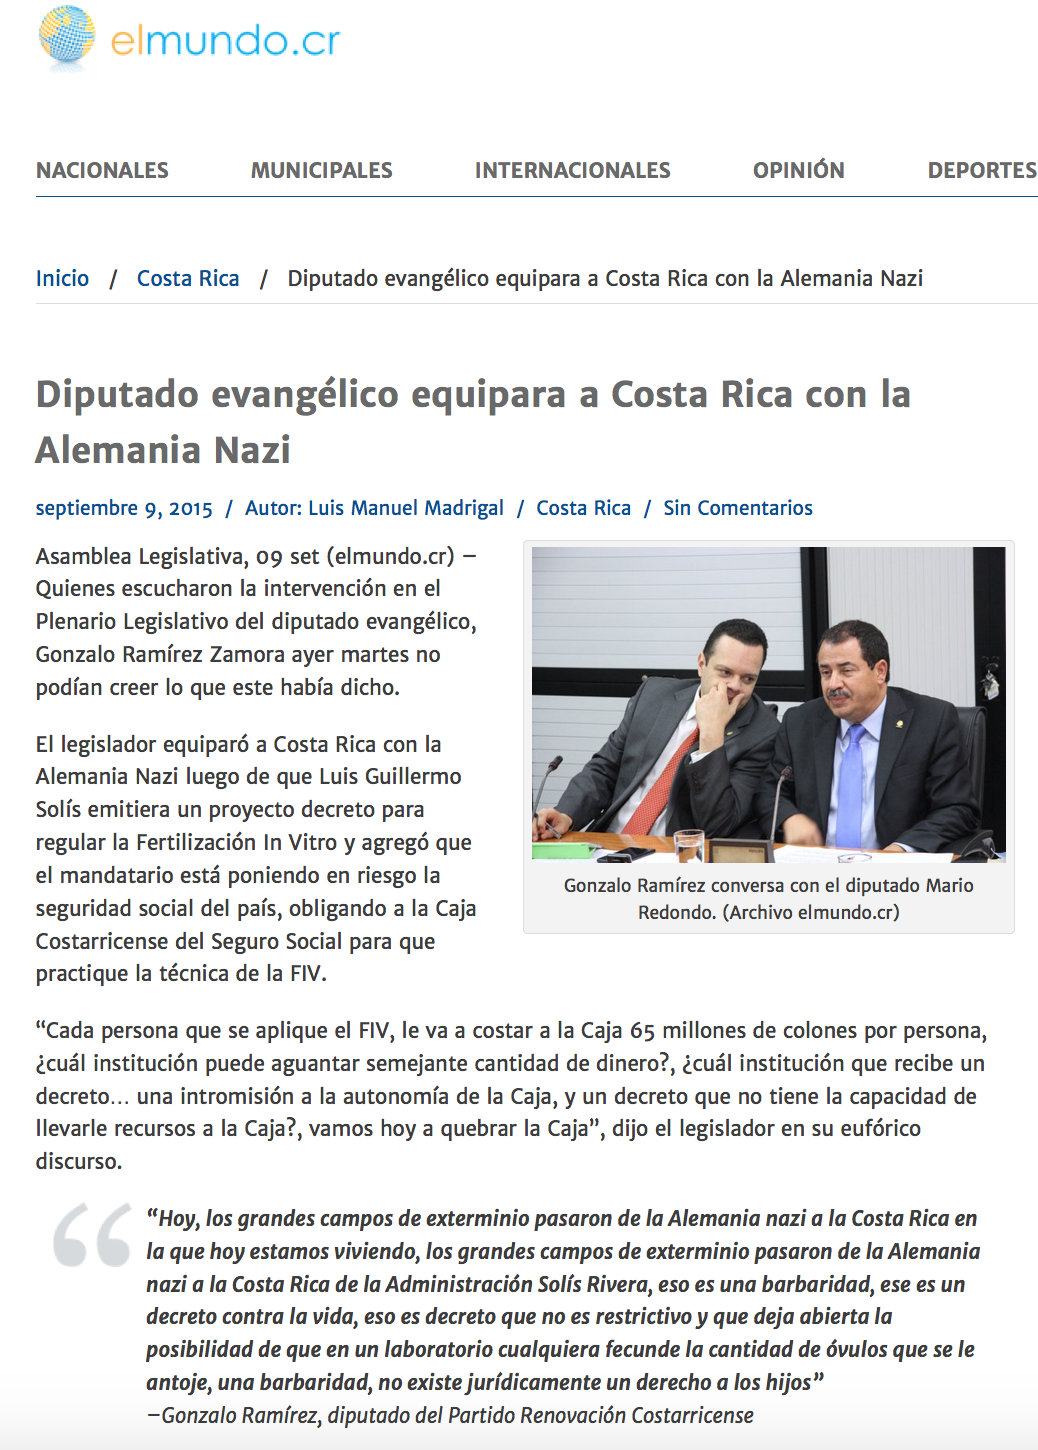
\includegraphics[width=15cm]{costarica-nazi-fiv}
    \captionof{figure}{Captura de pantalla de la noticia}
    \label{fig:falacia1}
\end{figure}

\newpage

\begin{table}[h!]
    \begin{tabular}{ll} 
        \toprule[1.5pt]
        Fuente & Periódico \href{http://elmundo.cr}{elmundo.cr}\\
        \midrule[0.5pt]
        Fecha  & 9 de setiembre 2015\\
        \midrule[0.5pt]
        Falacia & Palabras emotivas \\
        \bottomrule[1.5pt]
    \end{tabular} 
\end{table}

El legalización de la técnica de Fertilización in Vitro (FIV) ha resultado ser un tema muy polémico en nuestro país, principalmente en la asamblea legislativa en donde un pequeño grupo de diputados de partidos conservadores se oponen a la utilización de esta técnica aduciendo que atenta contra la vida humana.

En su discurso de la sesión del día martes 8 de setiembre del 2015, el diputado evangélico Gonzalo Ramírez Zamora, un claro opositor del FIV, llegó a comparar a Costa Rica con la Alamania Nazi diciendo que: \textit{``Hoy, los grandes campos de exterminio pasaron de la Alemania nazi a la Costa Rica en la que hoy estamos viviendo, los grandes campos de exterminio pasaron de la Alemania nazi a la Costa Rica de la Administración Solís Rivera, eso es una barbaridad, ese es un decreto contra la vida, eso es decreto que no es restrictivo y que deja abierta la posibilidad de que en un laboratorio cualquiera fecunde la cantidad de óvulos que se le antoje, una barbaridad, no existe jurídicamente un derecho a los hijos''}.

En su discurso el diputado Ramírez hace un claro uso de palabras emotivas con el fin de despertar sentimientos negativos ante la posible aprobación de esta técnica, de esta forma tanto diputados presentes, seguidores de su partido y público en general podrían llegar a crear sentimientos de miedo u odio con el fin de generar mayor oposición.

\noindent Dirección: \href{http://www.elmundo.cr/costarica/diputado-equipara-costa-rica-la-alemania-nazi-decreto-la-fiv/}{http://www.elmundo.cr/costarica/diputado-equipara-costa-rica-la-alemania-nazi-decreto-la-fiv/} \\
Discurso del diputado Ramírez: \href{https://www.youtube.com/watch?v=cK6AeaFB1Co}{https://www.youtube.com/watch?v=cK6AeaFB1Co}\\


\newpage
\section{Periodistas cuestionan a la costarricense del milagro sobre los incrédulos}

\begin{figure}[h]
    \centering
    
\includegraphics[width=15cm]{floribeth-mora-milagro}
    \captionof{figure}{Detalle de la noticia sobre el cuestionamiento del milagro de Floribeth Mora}
    \label{fig:falacia2}
\end{figure}

\newpage

\begin{table}[h!]
    \begin{tabular}{ll} 
        \toprule[1.5pt]
        Fuente & Periódico La Nación\\
        \midrule[0.5pt]
        Fecha  & 24 de abril 2014\\
        \midrule[0.5pt]
        Falacia & Peso de la prueba, inexplicado vs inexplicable, demostración por anécdota \\
        \bottomrule[1.5pt]
    \end{tabular} 
\end{table}


En el año 2011 Floribeth Mora, una ama de casa de 50 años residente en La Unión de Cartago, fue diagnosticada con un aneurisma en el lado izquierdo del cerebro. Luego de ser internada y de tener un estado de salud crítica, el aneurisma desapareció sin dejar rastro lo cual salvó Floribeth de la muerte. Ella aduce de que fue curada gracias a la intervención del fallecido Papa Juan Pablo II, el cual se le manisfestó por sueños. Esta historia logró trascender hasta llegar al Vaticano en donde luego de un estudio determinaron el caso de Floribeth calificaba como de milagro y gracias al mismo se concedió la beatificación del Papa.

En entrevistas y conferencias de prensa Floribeth manifestó de que: \textit{``Mi interés no está en convencer a los incrédulos. Dios me escogió y por su voluntad es que estoy acá. Lo importante es que esta loca, que ellos llaman, está sana''}. En estas declaraciones queda claro de que no se proporciona ninguna prueba que pueda ser refutada. Lo que se provee más bien es una especie de ``salida fácil'' ante los eventos por los cuales ella pasó. Se fabrica una explicación ``mágica'' que elimina cualquier proceso de razonamiento.

Esta noticia está disponible en:  \href{http://www.nacion.com/nacional/religion/Periodistas-cuestionan-costarricense-milagro-incredulos_0_1410459070.html?print=1}{http://www.nacion.com/nacional/religion/Periodistas-cuestionan-costarricense-milagro-incredulos\_0\_1410459070.html?print=1}

\newpage
\section{Jefa de prensa OIJ ganará ¢53 millones sin trabajar}

\begin{figure}[h!]
    \centering
    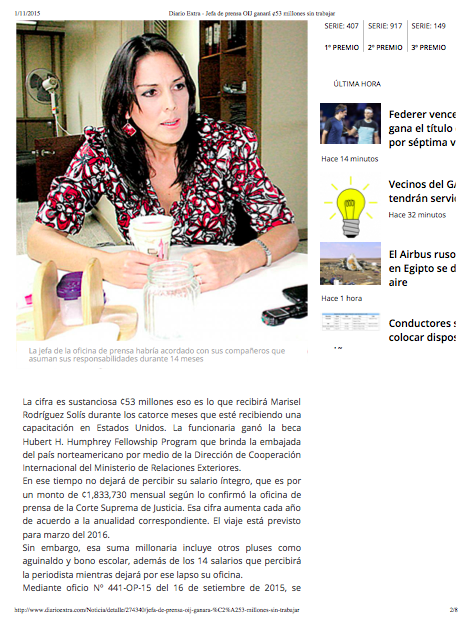
\includegraphics[width=15cm]{noticiaJefaOIJ}
    \captionof{figure}{Captura de pantalla noticia: Jefa de prensa OIJ ganará ¢53 millones sin trabajar}
    \label{fig:falacia3}
\end{figure}

\newpage

\begin{table}[h!]
    \begin{tabular}{ll} 
        \toprule[1.5pt]
        Fuente & Periódico La Extra\\
        \midrule[0.5pt]
        Fecha  & 1 de noviembre 2015\\
        \midrule[0.5pt]
        Falacia & Ad populum, palabras emotivas, falsas analogías. \\
        \bottomrule[1.5pt]
    \end{tabular} 
\end{table}

El artículo está redactado de una manera manipuladora para incentivar sentimientos de odio en la población.  El uso de frases como: ``sin trabajar'', ``suma millonaria'', ``todo pago'', ``no cumple requisitos'' dan una connotación negativa de a noticia desde el título y  sesgan la opinión del lector.

La misma noticia podría haberse presentado de manera positiva con solo cambiar la redacción. Por ejemplo haber incluyendo palabras como: ganar, oportunidad, orgullo y equidad de genero hubiesen generado en el lector sentimientos diferentes. 
Sería ideal que las noticias se redactaran de manera imparcial, y permitieran a los lectores decidir por si mismo su opinión. 

Esta noticia está disponible en: \href{http://www.diarioextra.com/Noticia/detalle/274340/jefa-de-prensa-oij-ganara-\%C2\%A253-millones-sin-trabajar}{http://www.diarioextra.com/Noticia/detalle/274340/jefa-de-prensa-oij-ganara-\%C2\%A253-millones-sin-trabajar}


\newpage
\section{¿Qué probabilidad de éxito dan los expertos a la Selección de Costa Rica}

\begin{figure}[h!]
    \centering
    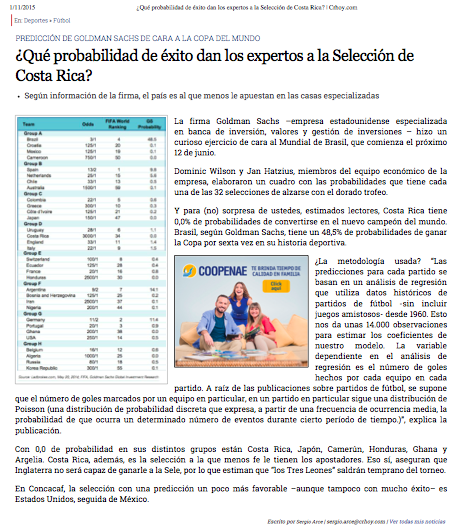
\includegraphics[width=15cm]{exitoSeleccion}
    \captionof{figure}{Captura de pantalla noticia: ¿Qué probabilidad de éxito dan los expertos a la Selección de
Costa Rica?}
    \label{fig:falacia4}
\end{figure}



\newpage
\begin{table}[h!]
    \begin{tabular}{ll} 
        \toprule[1.5pt]
        Fuente & Periódico \href{crhow.com}{crhoy.com}\\
        \midrule[0.5pt]
        Fecha  & 28 de mayo 2014\\
        \midrule[0.5pt]
        Falacia & Post Hoc, Ergo Propter Hoc \\
        \bottomrule[1.5pt]
    \end{tabular} 
\end{table}

El análisis que utilizan es el siguiente: como siempre les va mal $=$ les va a ir mal.

Basar la investigación en el número de goles hechos por cada equipo en el pasado no puede determinar la probabilidad de ganar de un equipo en el estado actual. No existe correlación, se trata más bien de una secuencia de eventos independientes.

Las razón reales de porque un equipo de futbol ha tenido un mal desempeño en el pasado no son analizadas. Razones como: mala condición física, poco entrenamiento, limitaciones económicas, mal entrenador, desmotivación entre otras,  pueden cambiar y un equipo de futbol de repente puede pasar de malo a bueno. De manera contraria un equipo de futbol puede de repente pasar de bueno a malo. Por lo tanto, consideramos que este estudio no tiene valor. 

Esta noticia está disponible en: \href{http://www.crhoy.com/cuantas-posibilidades-dan-los-expertos-a-la-seleccion-de-costa-rica-v2h3h7x}{http://www.crhoy.com/cuantas-posibilidades-dan-los-expertos-a-la-seleccion-de-costa-rica-v2h3h7x}

\newpage
\section{Fabio Chaves, sindicalista del ICE: ``Si la agresión de medios sigue, habrá respuesta''}

\begin{figure}[h!]
    \centering
    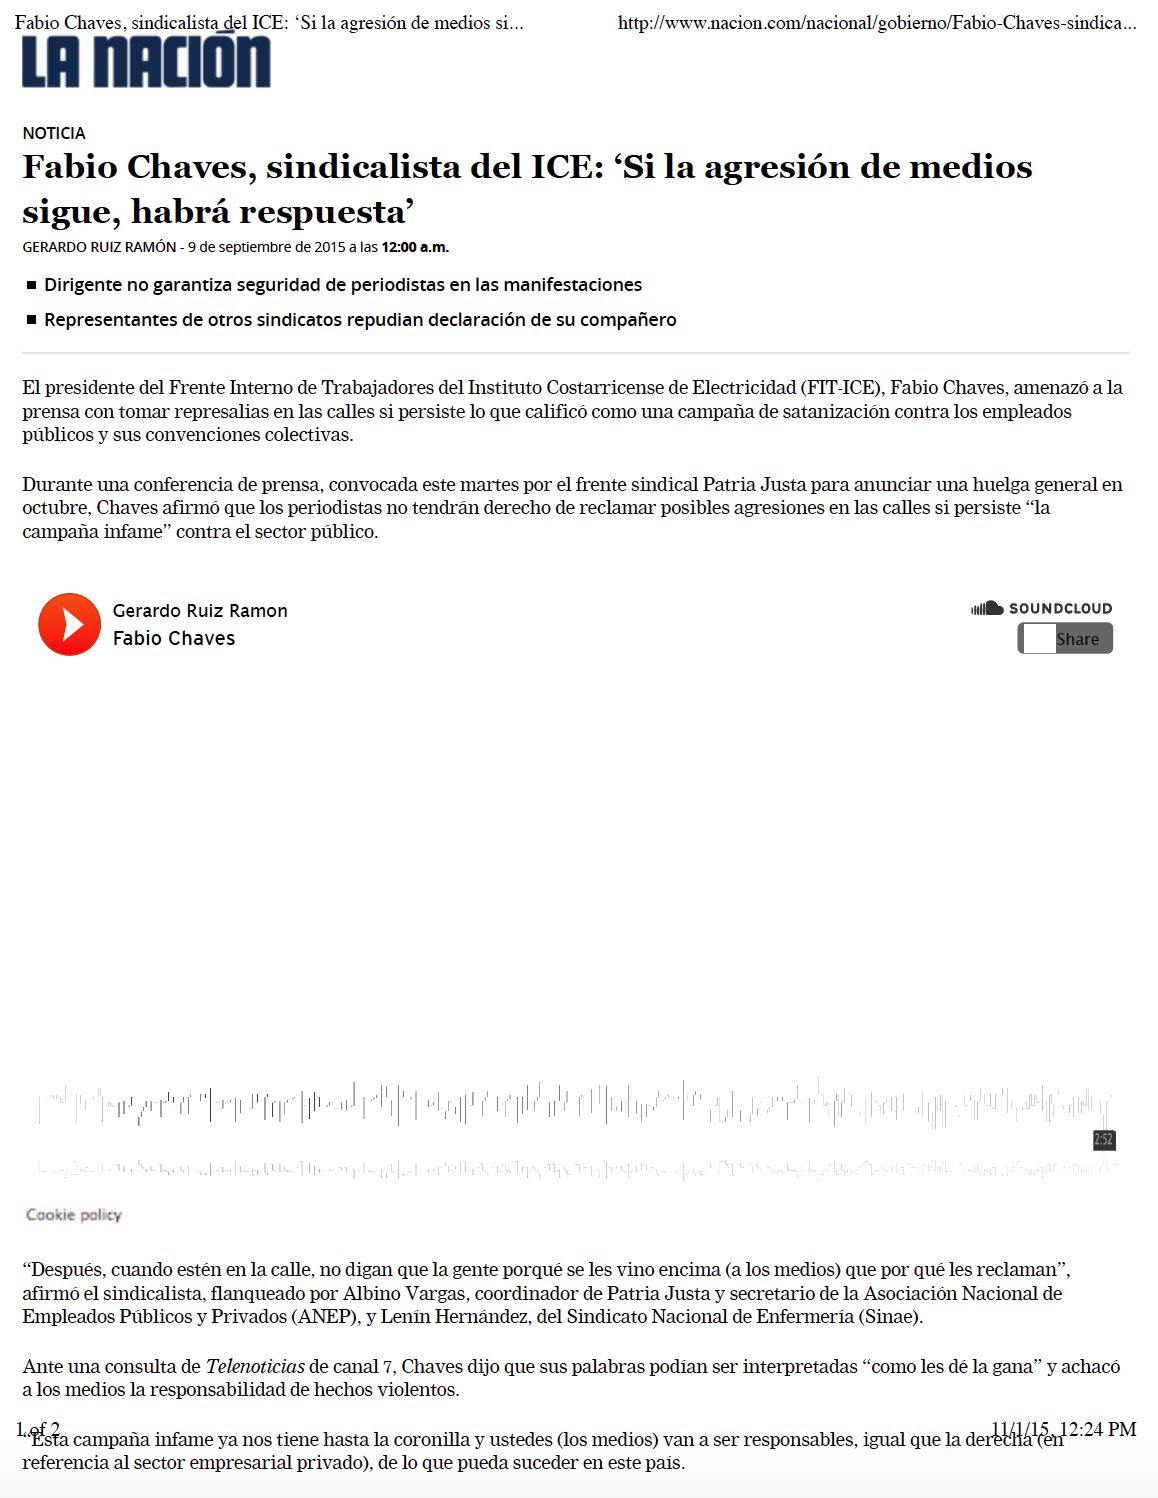
\includegraphics[width=15cm]{fabio-chaves-1}
    \captionof{figure}{Detalle de la noticia sobre la amenaza a la prensa de Fabio Chaves}
    \label{fig:falacia5-1}
\end{figure}

\begin{figure}[h!]
    \centering
    
\includegraphics[width=15cm]{fabio-chaves-2}
    \captionof{figure}{Detalle de la noticia sobre la amenaza a la prensa de Fabio Chaves}
    \label{fig:falacia5-2}
\end{figure}

\newpage
\begin{table}[h!]
    \begin{tabular}{ll} 
        \toprule[1.5pt]
        Fuente & Periódico La Nación\\
        \midrule[0.5pt]
        Fecha  & 9 de setiembre 2015\\
        \midrule[0.5pt]
        Falacia & \textit{Ad Hominen} \\
        \bottomrule[1.5pt]
    \end{tabular} 
\end{table}

Durante este año la discusión acerca de los salarios y beneficios de los empleados públicos ha sido intensa. Medios de comunicación radiales, televisivos y escritos han dado mucho cobertura al respecto .
El día martes 8 de setiembre en conferencia de presa, el presidente del Frente Interno de Trabajadores del Instituto Costarricense de Electricidad, Fabio Chaves amenazó a la prensa y al público en general con tomar acciones si se continuaban haciendo denuncias hacia los empleados públicos.

Chaves llegó a decir: \textit{``Después, cuando estén en la calle, no digan que la gente porqué se les vino encima que por qué les reclaman''}, más adelante añadió: \textit{``Porque, si somos agredidos, si somos atacados, vamos a responder, desde el punto de vista legal, pero, también, desde el punto de vista de la calle''}.

Lo anterior, es un caso de falacia de tipo \textit{Ad Hominen}. Fabio Chaves se dedicó en atacar a los medios presentes en la conferencia y a desprestigiar sus posiciones a base de amenazas. Casi y que se podría llegar a interpretar que el sindicalista estaba haciendo más un llamado ``a las armas'' en lugar de una  llamado a una huelga y, tomando en cuenta que esto viene de un líder sindical, las consecuencias a este llamado pudieron haber llegado a ser muy fuertes. 

\newpage
\section{Se cumplió la profecía en el Real Madrid, el técnico que no gana sale del equipo}

\begin{figure}[h!]
    \centering
    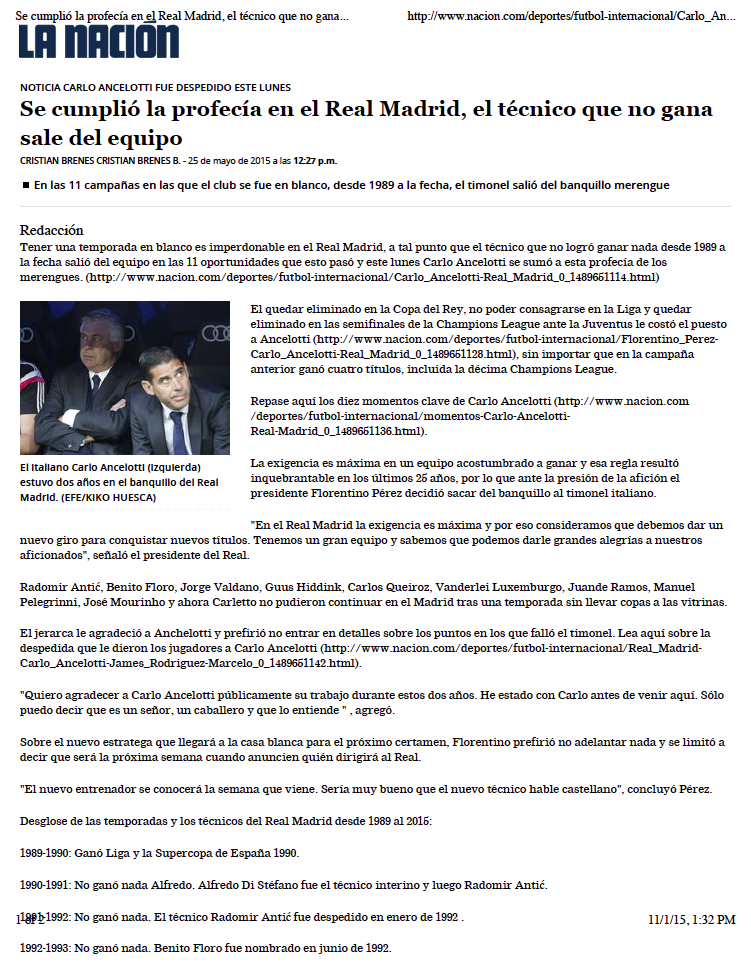
\includegraphics[width=17cm]{anchelotti-1}
    \captionof{figure}{Detalle de la noticia sobre despido de Carlo Anchelotti}
    \label{fig:falacia6-1}
\end{figure}

\begin{figure}[h!]
    \centering
    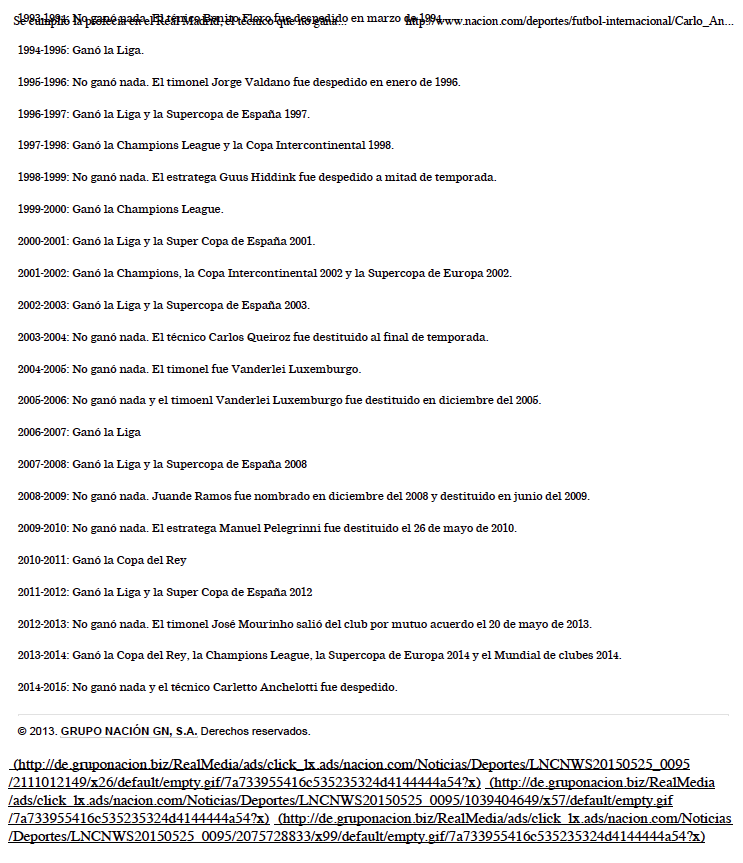
\includegraphics[width=16cm]{anchelotti-2}
    \captionof{figure}{Detalle de la noticia sobre despido de Carlo Anchelotti}
    \label{fig:falacia6-2}
\end{figure}

\newpage
\begin{table}[h!]
    \begin{tabular}{ll} 
        \toprule[1.5pt]
        Fuente & Periódico La Nación\\
        \midrule[0.5pt]
        Fecha  & 25 de mayo 2015\\
        \midrule[0.5pt]
        Falacia & Rumor y Realidad, representatividad \\
        \bottomrule[1.5pt]
    \end{tabular} 
\end{table}

En el mundo del fútbol el Real Madrid es probablemente el equipo más poderoso, siempre acostumbrado a exigir a sus jugadores y cuerpo técnico a rendir al máximo con el fin de la obteción de títulos, los cuales se van a traducir en mayor exposición, más fanáticos y más patrocinadores.
Esta gran exigencia a la que se sometido el equipo hace que la evaluación de sus jugadores y cuerpo técnico sea muy exhaustiva por lo que si se detecta un elemento que no da los resultados esperados este se podría llegar a separar. Por lo tanto, llegar a afirmar de que existe una ``profecía'' con respecto a la salida del entrenador Carlo Anchelotti por sus malos resultados no resulta ser un escenario nuevo en una institución como el Real Madrid. Los entrenadores son contratados y cesados de acuerdo a sus resultados.

Aunque el artículo provee un desglose del historial de los entrenadores del Real Madrid de 1989 a la fecha a modo de evidencia para confirmar de que cada vez que un entrenador no logró sus objectivos fue despedido, lo que expone no aporta nada ninguna cualdad premonitoria para asumir de que si un entrenador no logra el rendimiento esperado este va a ser despedido. De hecho, esta misma ``profecía'' se podría aplicar casi que a cualquier equipo deportivo competitivo.

Además podría existir un caso en el que por razones económicas o contractuales, un entrenador no llegue a ser despedido luego de tener malos resultados, esto se traería abajo esta predicción.

\newpage
\section{Luna roja, el eclipse que inquieta a los cristianos}

\begin{figure}[h!]
    \centering
    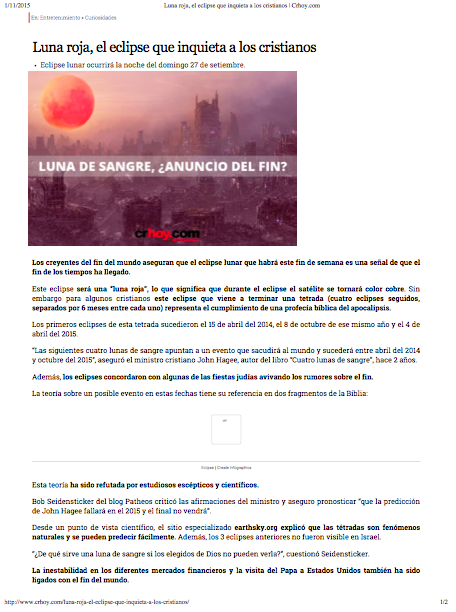
\includegraphics[width=15cm]{lunaRoja}
    \captionof{figure}{Captura de pantalla noticia: Luna roja, el eclipse que inquieta a los cristianos}
    \label{fig:falacia4}
\end{figure}

\newpage
\begin{table}[h!]
    \begin{tabular}{ll} 
        \toprule[1.5pt]
        Fuente & Periódico CRHoy\\
        \midrule[0.5pt]
        Fecha  & 24 de septiembre 2015\\
        \midrule[0.5pt]
        Falacia & Coincidencia, Inexplicado vs Inexplicable \\
        \bottomrule[1.5pt]
    \end{tabular} 
\end{table}

Los eclipses son eventos naturales, lo que sucede es que la luz de un cuerpo celeste es bloqueada por otro. Estos fenómenos no están asociados a ningún evento específico, ni son obras divinas. Que hubiesen cuatro eclipses seguidos separados por seis meses es producto de la casualidad o del rumbo de los astros, esto no implica de ninguna manera apocalipsis.  

Que el ministro cristiano John Hagee, autor del libro ``Cuatro lunas de sangre'' lo predijera hace dos años se debe a que posiblemente el evento ya fuera anunciado por los científicos o a la casualidad, después de todo que tan difícil es que se den cuatro eclipses en dos años. 

La noticia esta disponible en: \href{http://www.crhoy.com/luna-roja-el-eclipse-que-inquieta-a-los-cristianos}{http://www.crhoy.com/luna-roja-el-eclipse-que-inquieta-a-los-cristianos}


\newpage
\section{Rumor asegura que la tarde de este lunes iniciarán 96 horas de oscuridad }
\begin{figure}[h!]
    \centering
    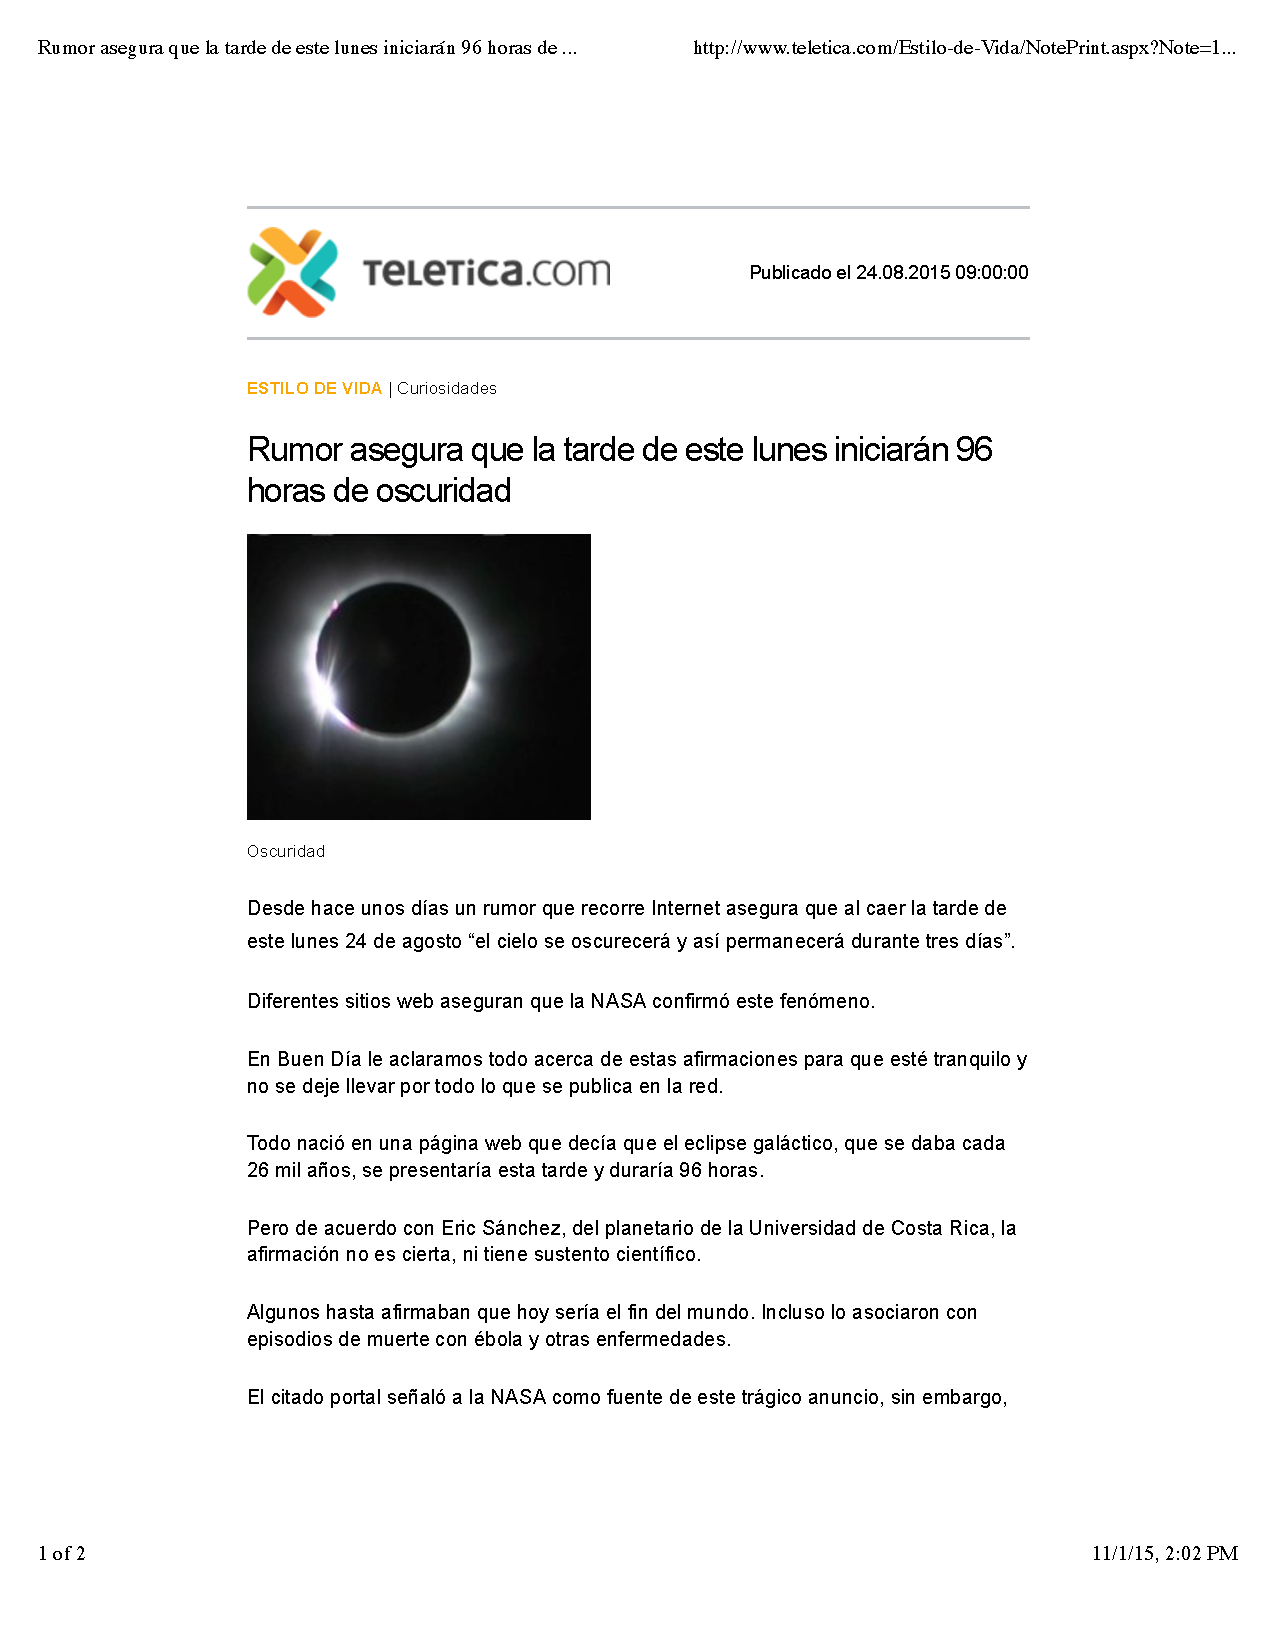
\includegraphics[width=17cm]{teletica-rumor}
    \captionof{figure}{Detalle de la noticia sobre el inicio de 96 horas de oscuridad}
    \label{fig:falacia2}
\end{figure}

\begin{table}[h!]
    \begin{tabular}{ll} 
        \toprule[1.5pt]
        Fuente & Teletica.com\\
        \midrule[0.5pt]
        Fecha  & 24 de agosto 2015\\
        \midrule[0.5pt]
        Falacia & Rumor y Realidad, Peso de la prueba \\
        \bottomrule[1.5pt]
    \end{tabular} 
\end{table}

Ver como se filtran este tipo de noticias en medios de comunicación colectiva resulta algo triste e indignante para muchos. Teletica.com y el programa ``Buen Día'' dan espacio a una nota generada a partir de un rumor en Internet de dudosa popularidad, es decir, ¿cuántas personas estaban realmente al tanto de esto? Si se llegara a saber que el cielo va a permaner oscuro durante tres días, este no sería un hecho que pasaría desapercibido dentro de la comunidad científica mundial.

Este tipo de notas son una muestra de cómo la obtención de mayores índices de \textit{ratings} en medios de comunicación llegan a ser lo más importante, sacrificando la calidad de los contenidos que son proporcionados.

\newpage
\section{De la bicibleta al BMW}
\begin{figure}[h!]
    \centering
    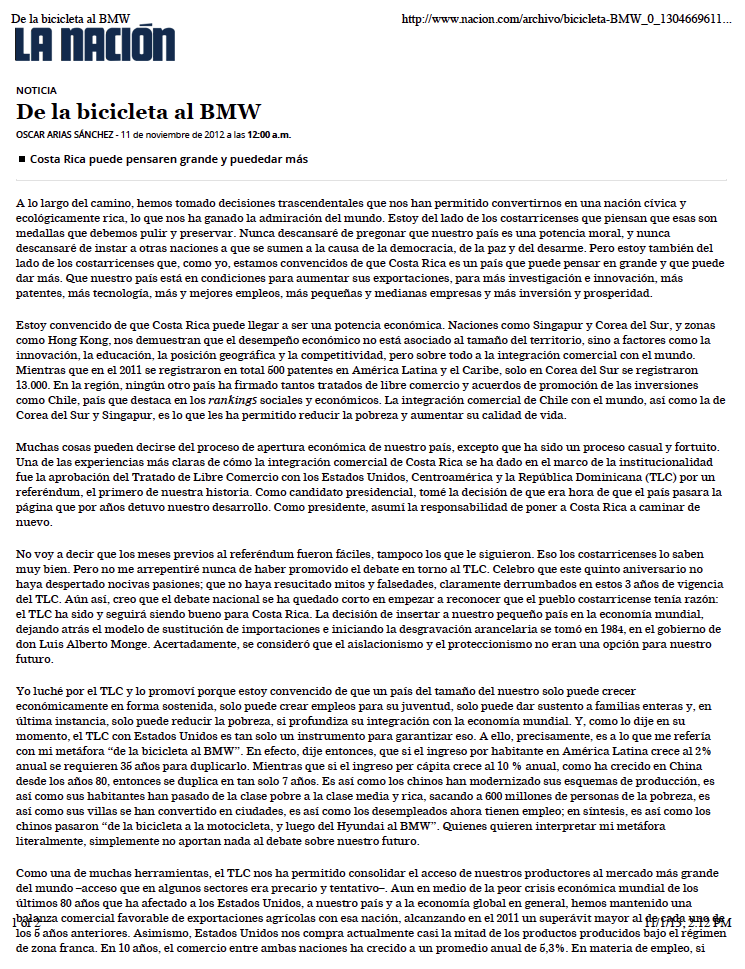
\includegraphics[width=16.5cm]{oscar-arias-bmw-1}
    \captionof{figure}{Editorial \textit{``De la bicibleta al BMW''}}
    \label{fig:falacia9-1}
\end{figure}

\begin{figure}[h!]
    \centering
    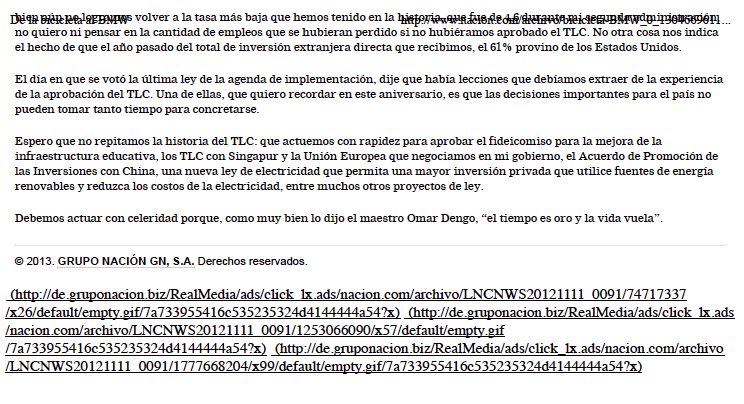
\includegraphics[width=16cm]{oscar-arias-bmw-2}
    \captionof{figure}{Editorial \textit{``De la bicibleta al BMW''}}
    \label{fig:falacia9-2}
\end{figure}

\begin{table}[h!]
    \begin{tabular}{ll} 
        \toprule[1.5pt]
        Fuente & Periódico La Nación\\
        \midrule[0.5pt]
        Fecha  & 11 de noviembre 2012\\
        \midrule[0.5pt]
        Falacia & Falacia de la Autoridad, Palabras emotivas \\
        \bottomrule[1.5pt]
    \end{tabular} 
\end{table}

Durante la campaña a favor del Tratado de Libre Comercio con los Estados Unidos (TLC), el expresidente Oscar Arias se dedicó a impulsar dicho tratado destacando el desarrollo y las grandes ventajas que traería para nuestro país. Durante esta campaña frases tales como las siguientes e convirtieron en el gancho para atraer la mayor cantidad de votantes pero además para crear una miedos e inseguridades a la población en caso de que este tratado no se aprobara.

\begin{itemize}
    \item
     \textit{``Los que hoy vienen en bicicleta, con el TLC vendrán en motocicleta BMW, y los que vienen en un Hyundai, vendrán en un Mercedes Benz, en esto consiste el desarrollo''}
     \item
     \textit{``Si quieren darle una cachetada a los gringos esta bien, pero el precio que tendrán que pagar por ello será muy caro, ya no será un tico que se lance del puente de los Anonos, sino miles''}
     \item
     \textit{``Los costarricenses con su voto reflejarán su confianza, de tal forma que quienes estén con el TLC es porque creen en mis propuestas y quienes respaldan el no es porque confían más en Albino Vargas.''}
     \item
     \textit{``Yo me comprometí a impulsar el TLC con EE.UU. y quiero decirles que si nos va mal, que si nos damos cuenta de que no hicimos lo correcto, pues simplemente nos salimos''}
    
\end{itemize}

Haciendose valer de su autoridad e influencia, este tipo de frases logró convencer a muchos votantes acerca del porqué habia que votar a favor del TLC ignorando cualquier otro tipo de evidencia o discusión al respecto\footnote{``Si lo dice Oscar Arias debe de ser verdad''}. Ocho años después de la firma de este tratado, se ha podido corroborar de que sus bondades no eran tantas y que los que manejaban bicicletas y Hyundais no fueron capaces de tener acceso a los ahnelados BMW y aunque en el artículo el expresidente aduzca de que de esta frase es utilizada más bien como una metáfora, lo cierto es que muchas personas (de zonas rurales, de bajos recursos o liberacionistas apasionados) no lo pudieron interpretar así y se lleguaron a creer ciegamente sus palabras.


\newpage
\section{La Nación anuncia el fallecimiento de Gustavo Cerati en 2010 }

\begin{figure}[h!]
    \centering
    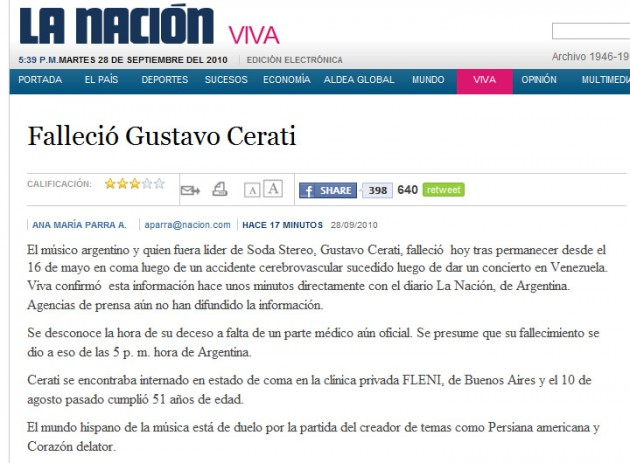
\includegraphics[width=14cm]{fallece-cerati}
    \captionof{figure}{Detalle de la noticia sobre el fallecimiento de Gustavo Cerati}
    \label{fig:falacia10}
\end{figure}

\begin{figure}[h!]
    \centering
    
\includegraphics[width=14.5cm]{cerati}
    \captionof{figure}{Detalle de la noticia sobre la disculpa de la muerte de Cerati}
    \label{fig:falacia10}
\end{figure}

\begin{table}[h!]
    \begin{tabular}{ll} 
        \toprule[1.5pt]
        Fuente & Periódico La Nación\\
        \midrule[0.5pt]
        Fecha  & 28 y 29 de setiembre del 2010\\
        \midrule[0.5pt]
        Falacia & Rumor y realidad, Falacia de la Autoridad\\
        \bottomrule[1.5pt]
    \end{tabular} 
\end{table}

No todo lo que escribe el periódico La Nación es cierto como muchos consideran. El 16 de mayo del año 2010, Gustavo Cerati apuraba la recta final de uno de sus conciertos en Caracas cuando, de repente, se desvaneció. El músico argentino había sufrido un derrame cerebral por obstrucción de la arteria carótida interna izquierda. Un respirador artificial mantuvo su corazón con vida durante cuatro años. Finalmente muere el 4 de setiembre del 2014.

En setiembre del 2010, La Nación publicó que el músico argentino había muerto, esto a raíz de una serie de rumores que surgieron alrededor del estado su salud, luego se pudo corroborar de que Cerati continuaba con vida (aunque en un estado muy delicado), esto obligó a La Nación a escribir una nota de disculpa para enmendar su error. Dos cosas estuvieron mal, una es que La Nación creyese el rumor y publicar información falsa. La otra es que la opinión publica creyera el rumor porque lo publicó La Nación. 

La nota principal ya no existe (aunque se pudo encontrar una captura de pantalla en un sitio externo a nacion.com) 
La nota de disculpa se puede encontrar en el siguiente link: 
\href{http://www.nacion.com/ocio/musica/Nacionem-pide-disculpas-informacion-Cerati_0_1149885065.html}{http://www.nacion.com/ocio/musica/Nacionem-pide-disculpas-informacion-Cerati\_0\_1149885065.html}

\newpage
\section{Diputado Óscar López le declara la guerra a la comunidad científica costarricense}

\begin{figure}[h!]
    \centering
    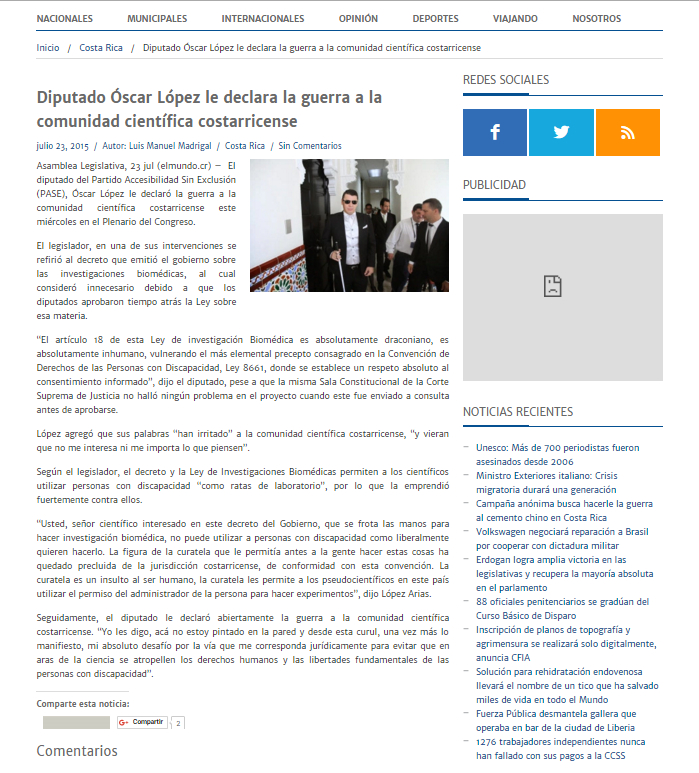
\includegraphics[width=14cm]{OscarLopez}
    \captionof{figure}{Captura de pantalla Noticia de Óscar Lopez}
    \label{fig:falacia11}
\end{figure}

\newpage
\begin{table}[h!]
    \begin{tabular}{ll} 
        \toprule[1.5pt]
        Fuente & Periódico \href{http://www.elmundo.cr}{elmundo.cr}\\
        \midrule[0.5pt]
        Fecha  & 23 julio 2014\\
        \midrule[0.5pt]
        Falacia & Peso de la prueba\\
        \bottomrule[1.5pt]
    \end{tabular} 
\end{table}

En este caso el diputado Óscar López tiene una hipótesis, él piensa que los  científicos van a utilizar personas con discapacidad ``como ratas de laboratorio'' pero no tiene ninguna prueba al respecto y ni se esfuerza por demostrar su hipótesis. 

Acusa que lo científicos están frotándose las manos por hacer pruebas con personas con discapacidad, pero es una acusación vacía, sin pruebas y sin validez. El esfuerzo por demostrar lo que está diciendo y dar validez a su argumento le corresponde únicamente a él.   

La noticia completa la puede encontrar en: \href{http://www.elmundo.cr/costarica/diputado-oscar-lopez-le-declara-la-guerra-a-la-comunidad-cientifica-costarricense/}{http://www.elmundo.cr/costarica/diputado-oscar-lopez-le-declara-la-guerra-a-la-comunidad-cientifica-costarricense}

\newpage
\section{Justo Orozco sobre homosexuales: ``Si no se les ve el plumero, no sé quiénes son''}

\begin{figure}[h!]
    \centering
    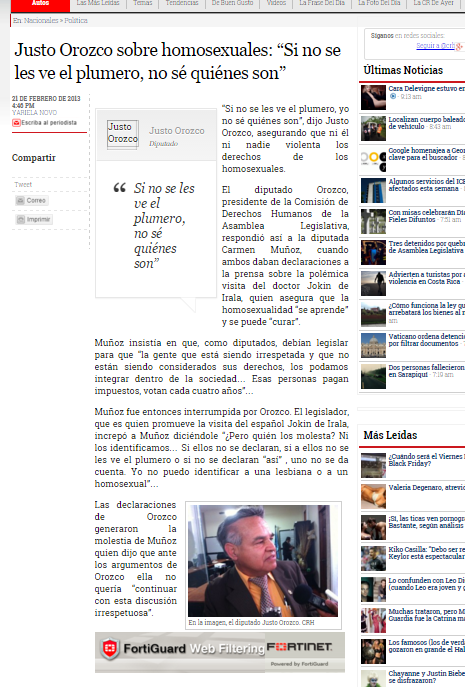
\includegraphics[width=14cm]{justo}
    \captionof{figure}{Captura de pantalla Noticia de Justo Orozco}
    \label{fig:falacia12}
\end{figure}

\newpage
\begin{table}[h!]
    \begin{tabular}{ll} 
        \toprule[1.5pt]
        Fuente & Periódico \href{http://crhoy.com}{crhoy.com}\\
        \midrule[0.5pt]
        Fecha  & 21 febrero 2013\\
        \midrule[0.5pt]
        Falacia & Generalización, \textit{Ad Hominen}\\
        \bottomrule[1.5pt]
    \end{tabular} 
\end{table}

En este caso Justo Orozco generaliza casos aislados. Se asume que cuando se refiere a ``se le ve el plumero'', se está hablando sobre hombres homosexuales con conductas femeninas. 

En este caso Justo sugiere que todos los hombres afeminados son homosexuales y además que está en una forma para identificar a los homosexuales de los heterosexuales. 
Esto es una generalización apresurada, la hipótesis de Justo no puede ser validad porque da como regla general un hecho por medio de la observación de algunos casos. Otra característica reconocible en este comentario es el desprestigio hacia la comunidad homosexual por parte de este diputado.



%\begin{thebibliography}{9}
%
%\bibitem{R1} Kopka~H, Daly~PW. 2003. \emph{A Guide to \LaTeX} (4th~edn).
%Addison-Wesley.
%
%\bibitem{R2} Lamport~L. 1994. \emph{\LaTeX: a Document Preparation System} (2nd~edn).
%Addison-Wesley.
%
%\bibitem{R3} Mittelbach~F, Goossens~M. 2004. \emph{The \LaTeX\ Companion}
%(2nd~edn). Addison-Wesley.
%\end{thebibliography}


\end{document}

